\documentclass[14pt, a4paper]{article}
\usepackage[russian]{babel}
\usepackage{graphicx}
% \usepackage{tabularx}
\usepackage{layout}
\usepackage[14pt]{extsizes}
\usepackage[hidelinks]{hyperref}
\usepackage{caption}

\usepackage{listings}
\usepackage{xcolor}
\usepackage{float}
\usepackage{ulem}

\setcounter{tocdepth}{4}
\setcounter{secnumdepth}{4}
\setlength{\emergencystretch}{5pt}
% \usepackage[compact]{titlesec}

\oddsidemargin = 0pt
\marginparwidth = 45pt %57
\textwidth = 467pt
\textheight = 716pt
\topmargin = 0pt %17
\footskip = 30pt %30
\headheight = 0pt %12
\headsep = 0pt %25

\title{Методичка 4}

\definecolor{codegreen}{rgb}{0,0.6,0}
\definecolor{codegray}{rgb}{0.5,0.5,0.5}
\definecolor{codepurple}{rgb}{0.58,0,0.82}
\definecolor{backcolour}{rgb}{0.97,0.97,0.97}

\lstdefinestyle{mystyle}{
    backgroundcolor=\color{backcolour},   
    commentstyle=\color{codegreen},
    keywordstyle=\color{magenta},
    numberstyle=\tiny\color{codegray},
    stringstyle=\color{codepurple},
    basicstyle=\ttfamily\footnotesize,
    breakatwhitespace=false,         
    breaklines=true,                 
    captionpos=b,                    
    keepspaces=true,
    frame=single,                 
    % numbers=left,                    
    % numbersep=5pt,                  
    showspaces=false,                
    showstringspaces=false,
    showtabs=false,                  
    tabsize=2,
    extendedchars=\true,
    inputencoding=utf8x
}

\lstdefinelanguage{docker}{
  keywords={FROM, RUN, COPY, ADD, ENTRYPOINT, CMD,  ENV, ARG, WORKDIR, EXPOSE, LABEL, USER, VOLUME, STOPSIGNAL, ONBUILD, MAINTAINER},
  keywordstyle=\color{blue}\bfseries,
  identifierstyle=\color{black},
  sensitive=false,
  comment=[l]{\#},
  commentstyle=\color{purple}\ttfamily,
  stringstyle=\color{red}\ttfamily,
  morestring=[b]',
  morestring=[b]"
}

\lstset{style=mystyle}


\begin{document}

\begin{titlepage}
    \topmargin=216pt
    \newpage
    \hangindent=0.7cm
    \huge ИУ-10\\
    Системное\\
    Программное\\
    Обеспечение\\
    \textbf{Администрирование Linux\\ 
    Введение в Linux. Философия, базовые
понятия, установка дистрибутива}

    \vspace{10cm}

    \begin{center}
        \small\textit{Москва, 2022}
    \end{center}
\end{titlepage}

\tableofcontents
\section*{На этом уроке}
\addcontentsline{toc}{section}{На этом уроке}
\begin{enumerate}
    \item Обсудим, что такое Linux и почему он стал таким популярным.
    \item Посмотрим, какие типы дистрибутивов ОС Linux существуют. Научимся выбирать дистрибутив
    операционной системы под свои нужды. Узнаем, в чём основное различие между
    RеdHat-подобными и Debian-подобными ОС.
    \item Познакомимся с инструментами виртуализации VirtualBox и VmWare Player
    \item Создадим виртуальную машину и проведем установку ОС Linux
\end{enumerate}
\newpage





\section*{Введение}
\addcontentsline{toc}{section}{Введение}
Linux — известная серверная операционная система. Большинство веб-сайтов и веб-сервисов
работают именно на ней. Независимо от того, какой язык используется для реализации сервиса —
PHP, Python или JavaScript — скорее всего, система работает под управлением Linux. Большой набор
программного обеспечения, выполняющего функции сетевых узлов (балансировщики трафика,
прокси-серверы и даже маршрутизаторы), также функционирует в среде Linux. Если Вы планируете
разрабатывать решения в одном из вышеперечисленных направлений, Вы должны иметь
представление о том, как функционирует операционная система в настоящее время. Поэтому, если
для повседневной работы Вы используете Windows, хорошим решением будет использование
виртуальной машины с такой же операционной системой, что будет работать в production.

В крупных компания настройкой операционных систем занимаются системные
администраторы, но вам нужно в общих чертах понимать, как это делается, и суметь настроить для
домашнего использования. Это ускорит вашу работу, так как базовые проблемы вы сможете решить
быстро сами, если потребуется установить какой-то софт, то вы тоже сможете с этим справится.

Специалист по информационной безопасности сможет найти изъяны в системе, построенной
на основе серверов Linux. Кроме того, для использования профессиональных инструментов, которые
предназначены для работы в Linux, необходимо знакомство с операционной системой.

Есть облачные решения и для Data Science. В основном они базируются как раз на
Linux-машинах, благодаря стабильности и надежности операционной системы.

Отдельно стоит упомянуть разработчиков iOS. Система Mac OS основана на UNIX, как и
GNU/Linux. Многое, что есть в Linux, есть и в MAC OS X. Кроме того, Mac OS непосредственно
содержит компоненты GNU (bash и утилиты). Для работы с Xcode необходимо знакомство с системой.

\subsection*{Кому курс полезен}
\addcontentsline{toc}{subsection}{Кому курс полезен}
\begin{itemize}
    \item \textit{Системным администраторам}. В особенности, если планируете администрировать
    UNIX-подобные системы.
    \item \textit{Веб-разработчикам}. Хотя, как правило, веб-разработка не требует глубоких познаний Linux и
    TCP/IP, понимание системы, под которой вы работаете, делает вас квалифицированным и
    дорогостоящим специалистом.
    \item \textit{iOS-разработчикам}. Вы научитесь лучше понимать систему, которая, как и Linux,
    UNIX-подобна и содержит GNU-компоненты.
    \item \textit{Разработчикам решений для Linux}: системным программистам, прикладным программистам,
    разработчикам любых решений, для которых Linux — родная среда выполнения.
    \item \textit{Инженерам}, использующим Linux для встраиваемых и промышленных систем.
    \item \textit{Тестировщикам}. Специалистам данной профессии необходимо уметь работать в среде, где
    они будут запускать тестируемое приложение.
    \item \textit{Специалистам ИИ, Data Science, Big Data}, так как такие вычисления производятся, как
    правило, на Linux-машинах.
    \item \textit{Специалистам по компьютерной безопасности}.
    \item \textit{Системным инженерам DevOps}. Развертывание и деплой высоконагруженных сервисов, как
    правило, осуществляется на Linux-кластерах.
\end{itemize}
\newpage


\section*{Что такое Linux}
\addcontentsline{toc}{section}{Что такое Linux}
\subsection*{UNIX way}
\addcontentsline{toc}{subsection}{UNIX way}
Философия Unix, известная как UNIX way, является подходом, которому следует архитектура
UNIX-подобных систем, а Linux является именно такой. Есть несколько разных определений, что
такое UNIX way, при этом среди них можно выделить несколько важных принципов. Среди них мы
отметим:
\begin{itemize}
    \item Утилиты — маленькие отлаженные программы, решающие только свою (и, зачастую,
    единственную) задачу.
    \item Более сложные задачи можно решать, комбинируя утилиты, запуская их с помощью
    конвейеров.
    \item Конфигурационные файлы хранятся в виде простых текстовых файлов.
    \item Все есть файл.
\end{itemize}

Благодаря использованию потоков и возможности работы с устройствами как файлами, для
таких маленьких шустрых программ можно совмещать прием и передачу данных, тем самым
добиваясь гибкости.

Принципы UNIX вы будете использовать при работе Linux и наблюдать воочию постоянно.\\

\subsection*{Операционная система Linux}
\addcontentsline{toc}{subsection}{Операционная система Linux}
Linux или GNU/Linux — популярная операционная система (ОС), которая распространена как
серверная ОС, так и все больше используется для персональных компьютеров. Одно из главных
свойств и достоинств операционной системы — открытый исходный код. В связи с этим часто
появляются и применяются компоненты, разработанные независимыми людьми и группами
разработчиков.

Если быть точным, Linux — это целое семейство операционных систем, базирующихся на:
\begin{itemize}
    \item \textbf{GNU} — UNIX-подобное операционное окружение, которое состоит из утилит, операционной
    оболочки и ее команд, а также средств разработки, прежде всего, ‒ коллекции компиляторов
    gcc;
    \item \textbf{Linux} — ядро операционной системы, по имени которого часто называется и вся ОС.
\end{itemize}
Если в ОС Linux используется графический режим, появляется еще один компонент:
\begin{itemize}
    \item \textbf{X Windows System} — оконная система, привычная по работе с ОС Windows.
\end{itemize}
На Рис.1 в общем виде изображена архитектура операционной системы. В центре
располагается один из самых важных ее элементов - Kernel или упомянутое ранее ядро. Ядро - это
программа, лежащая в основе операционной системы компьютера, основной задачей которой
является контроль доступа к аппаратным ресурсам. Код ядра всегда выполняется процессором на
привилегированном (по сравнению с пользовательскими процессами) уровне. Для пользователя эта
часть системы прозрачна, зато программисты активно используют функции ядра, называемые
системными вызовами (System Call) при написании программ. Ядро преобразует системные вызовы в
сигналы, понятные аппаратным ресурсам, и взаимодействует с оборудованием посредством
встроенных или динамически подгружаемых драйверов. Системные вызовы и модули (части
программы) ядра исполняются в пространстве ядра (Kernel Space).

\begin{figure}[h]%current location
    \centering
    \scalebox{0.7}{
\includegraphics[width=1\textwidth]{imgs/1.0.png}}
    \caption{\textit{Архитектура ОС}\\}
    \label{1.0} %framework,fig1
\end{figure}

Под пользовательским пространством (User Space) понимается весь код в операционной
системе, который находится вне ядра и только взаимодействует с ним с помощью системных вызовов.
Большинство Unix-подобных операционных систем (включая Linux) поставляются с набором утилит,
языков программирования и графических инструментов, являющимися приложениями
пользовательского пространства.

Вокруг наименования существует спор. Наиболее распространенные варианты:

\begin{itemize}
    \item \textbf{Linux}. Подразумевается, что не только ядро носит такое название, но и все семейство ОС
    целиком;
    \item \textbf{GNU/Linux}. На этом варианте настаивает Ричард Столлман, основатель проекта GNU. Он
    подчеркивает, что операционная система — не только ядро, но и многие важные компоненты,
    которые в ней используются, в частности, проект GNU.
\end{itemize}
У каждого из подходов есть аргументы как за, так и против. Существуют операционные
системы на ядре Linux, в которых нет GNU: Android или Open webOS. Кроме того, ОС — не только
ядро Linux и окружение GNU, но и множество других компонентов: X Windows System, Systemd и т.д.
Полное их перечисление сделало бы название слишком громоздким.

Мы будем считать наименования Linux и GNU/Linux синонимами. Когда будет идти речь о ядре
Linux, укажем на это отдельно.\\


\subsubsection*{Популярные операционные системы Linux}
\addcontentsline{toc}{subsubsection}{Популярные операционные системы Linux}

Всё богатство мира дистрибутивов Linux можно разделить на несколько типов:

\begin{enumerate}
    \item Дистрибутивы, основанные на ОС Debian (Ubuntu, Mint и т. д.).
    \item Дистрибутивы, основанные на ОС Red Hat (CentOS, Fedora, Oracle Linux).
    \item Отдельно, несмотря на то, что есть схожесть с типом пакетного менеджера RPM c Red Hat,
    можно выделить дистрибутивы SUSE и OpenSUSE.
    \item Все остальные: Slackware, Gentoo, Arch Linux и многие другие.
\end{enumerate}

Это абсолютно условное деление на группы, основанное на двух составляющих:

\begin{enumerate}
    \item Пакетный менеджер и формат пакетов.
    \begin{itemize}
        \item dpkg (расширение файлов .deb, для удобства работы используется apt) — в
        основанных на Debian дистрибутивах (но не обязательно, система может быть
        привнесена и в дистрибутивы иного происхождения);
        \item rpm (расширение файлов .rpm, для удобства работы используется yum) — в
        основанных на Red Hat дистрибутивах.
    \end{itemize}
    \item Общий дистрибутив-предок. Как говорилось ранее, для Ubuntu и Mint общим предком является
    \href{https://www.debian.org/}{Debian}, а для Centos и Oracle Linux — \href{https://www.redhat.com/en}{Red Hat Linux}.
\end{enumerate}

Более подробная информация о существующих типах дистрибутивов Linux есть \href{https://distrowatch.com/}{на сайте
DistroWatch}.

Наш курс будет основан на изучении \href{https://ubuntu.com/}{дистрибутива Ubuntu}. Ubuntu — один из наиболее
популярных продуктов как для домашнего использования, так и для серверных решений. Основные
два варианта дистрибутива: Ubuntu Desktop и Ubuntu Server. Desktop версия от Server отличается
только наличием набора программного обеспечения, который необходим обычному пользователю ПК:
удобная графическая оболочка, видео- и аудиоплееры, простейшие программы для просмотра фото,
офисные приложения.

Дистрибутив Ubuntu прекрасно задокументирован: практически на любой вопрос вы можете
найти ответ либо в официальной документации, либо на страницах сообществ. Дистрибутив
регулярно обновляется и зарекомендовал себя как стабильная операционная система. Для получения
наиболее актуальной версии ОС Ubuntu необходимо перейти на официальный сайт в раздел
\href{https://ubuntu.com/#download}{Download}, и дальше вам предстоит выбрать версию.

\subsection*{Версии}
\addcontentsline{toc}{subsection}{Версии}

На момент в обоих типах нам доступны две версии. Это 20.x LTS — версии дистрибутива с
длительной поддержкой (LTS — сокр. от англ. Long Term Support), то есть данные дистрибутивы будут
получать обновления достаточно долгое время, порядка пяти лет. Дистрибутив включает в себя
только стабильные пакеты. Версии LTS выпускаются раз в два года. Не LTS версии содержат в себе
версии пакетов, которые не попадают в LTS версию из-за их возможной нестабильности. Версии
выпускают где-то каждые девять месяцев, и они включают в себя самые новые пакеты.

Для домашнего или рабочего ПК вполне допустимо, даже лучше, использовать не LTS версии,
а вот для сервера рекомендуется использовать LTS хотя бы из соображений стабильности.

\textbf{Внимание!} \textit{\uline{Вы можете использовать любой удобный для вас дистри\-бутив, но в рамках
курса мы будем работать с последней доступной LTS версией Ubuntu Server}}.



\section*{Виртуализация}
\addcontentsline{toc}{section}{Виртуализация}

Виртуализация — механизм, который позволяет гибко использовать аппаратные возможности
машины. Виртуализация позволяет запускать на одном компьютере несколько параллельно
исполняющихся операционных систем, более того, в работе несколько виртуальных машин выглядят
аналогично, как если бы работали несколько аппаратных машин. Это достигается, в частности,
благодаря предоставлению гипервизором (в нашем случае домашним персональным компьютером)
интерфейса доступа к оборудованию.

\begin{figure}[h]%current location
    \centering
    \scalebox{0.7}{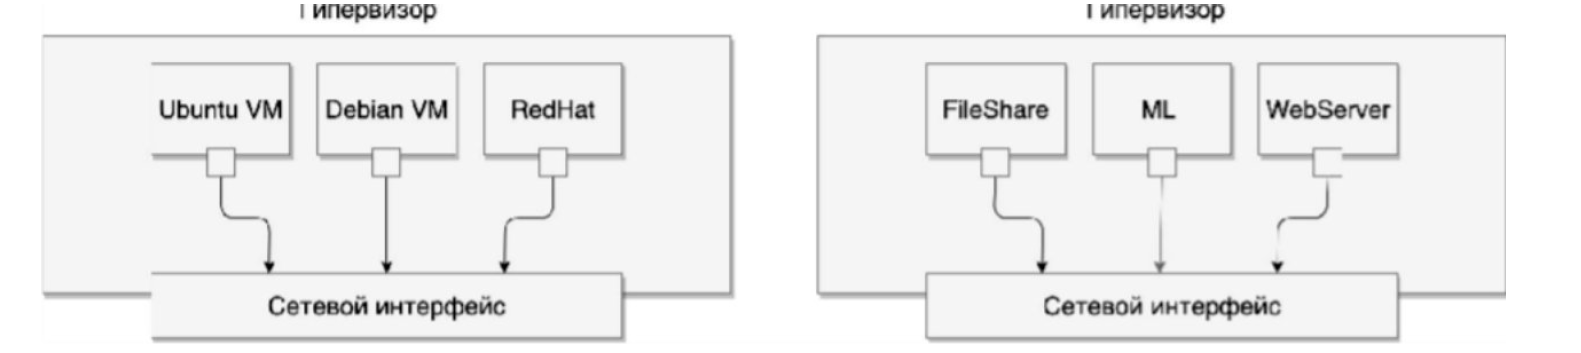
\includegraphics[width=1\textwidth]{imgs/1.1.png}}
    \caption{Виртуализация\\}
    \label{1.1} %framework,fig1
\end{figure}

Как правило, виртуальные машины наделяются IP-адресами («серыми» или «белыми», в
зависимости от задач), что позволяет взаимодействовать виртуальным машинам между собой, хостам
и виртуальным машинам, виртуальным машинам и любым другим, в локальной сети или интернете,
если туда есть доступ. Обращаясь к удаленному компьютеру по адресу 5.61.239.22, вы даже не
знаете, это адрес на физического сервера или виртуальной машины.

\textbf{Важно:} \textit{\uline{Крайне не рекомендуется для изучения Linux сносить вашу операционную систему
(так как можно не суметь ее полноценно на\-строить, удалить по ошибке важные данные, а также
не суметь прослу\-шать вебинар) Для обучения установите VMWare Player или VirtualBox.}}

\subsection*{Создание виртуальной машины}
\addcontentsline{toc}{subsection}{Создание виртуальной машины}

Для начала работы нам необходимы следующие инструменты:

\begin{enumerate}
    \item Готовая виртуальная машина со следующими параметрами: ЦПУ — 1, ОЗУ — 2 GB, жёсткий
    диск — не менее 10 GB. \textbf{Важно!} \textit{\uline{Создание и настройку виртуальной машины в VirtualBox и
    VMware для целей курса вы можете \href{https://docs.google.com/presentation/d/1142W3Wj-WKgfZX0TrA78y17ofYg-OYV_ljYhe79wMcU/edit}{посмотреть по ссылке}}}.
    \item Скачанный образ последней LTS версии Ubuntu Server или Ubuntu Desktop.
\end{enumerate}

Подключаем образ к виртуальной машине, как это показано в инструкции и запускаем её.



\section*{Обзор главного окна инсталлятора}
\addcontentsline{toc}{section}{Обзор главного окна инсталлятора}
\textbf{Примечание!} \textit{\uline{Все опции установки, предлагаемые инсталлятором, из\-на\-чально применимы
и в большинстве случаев оптимальны, с ними можно просто соглашаться. Далее мы рассмотрим
моменты, на ко\-то\-рые стоит обратить свое внимание, но опять же изменять не обя\-за\-тель\-но.}}

\begin{figure}[h]%current location
    \centering
    \scalebox{0.9}{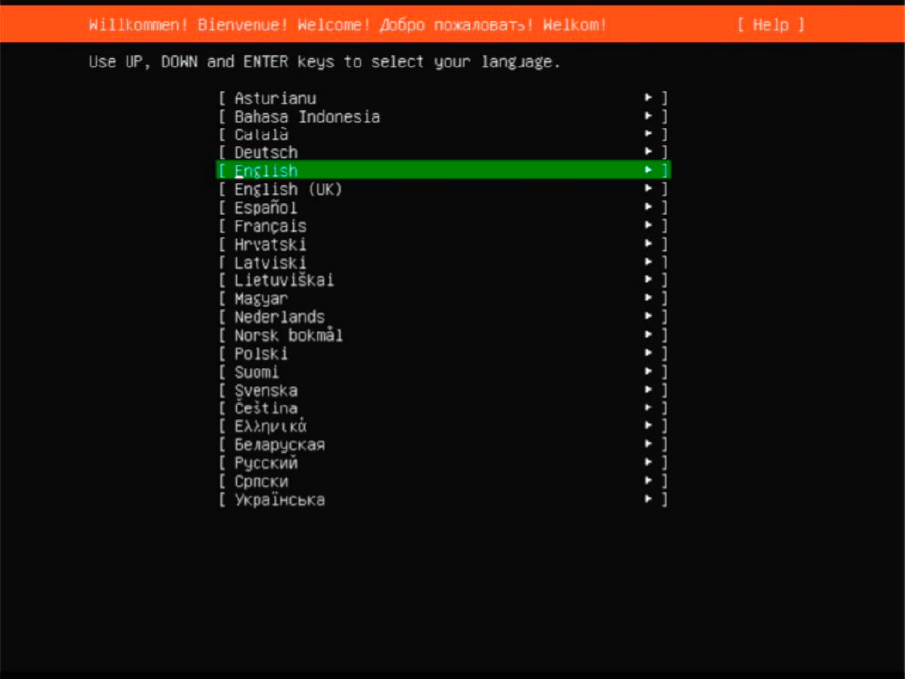
\includegraphics[width=1\textwidth]{imgs/1.2.png}}
    \label{1.2} %framework,fig1
\end{figure}
\textbf{\uline{ВАЖНО! УСТАНАВЛИВАЙТЕ ТОЛЬКО АНГЛИЙСКУЮ ВЕРСИЮ ОПЕРАЦИОННОЙ СИСТЕМЫ!}}

После старта мы увидим первое отличие серверной версии Ubuntu от десктопной —
отсутствие графического интерфейса у инсталлятора. Управление простое: клавиши «Вверх», «Вниз»,
«Влево», «Вправо» — перемещение по меню, клавиша «Пробел» — выбор пункта, Enter применяет
выбранное.

Первый шаг — выбор языка системы. Здесь оставляем английский язык, выбираем клавишу
«Готово» и переходим к пункту настройки сети.\\


\subsection*{Настройка сети}
\addcontentsline{toc}{subsection}{Настройка сети}

Выбираем сетевой интерфейс и жмём Enter. Нам предлагается несколько путей назначения
IP-адреса нашему серверу:

\begin{enumerate}
    \item Используя протокол DHCP (Automatic DHCP) — автоматическое назначение IP адреса.Этот
    вариант наиболее удобен, поэтому выберем его.
    \item Вручную (Manual) — используется, когда мы знаем настройки сети для нашего сервера
    \item Отключена (Disabled) — вариант, когда сеть не используется.
\end{enumerate}

\begin{figure}[h]%current location
    \centering
    \scalebox{0.8}{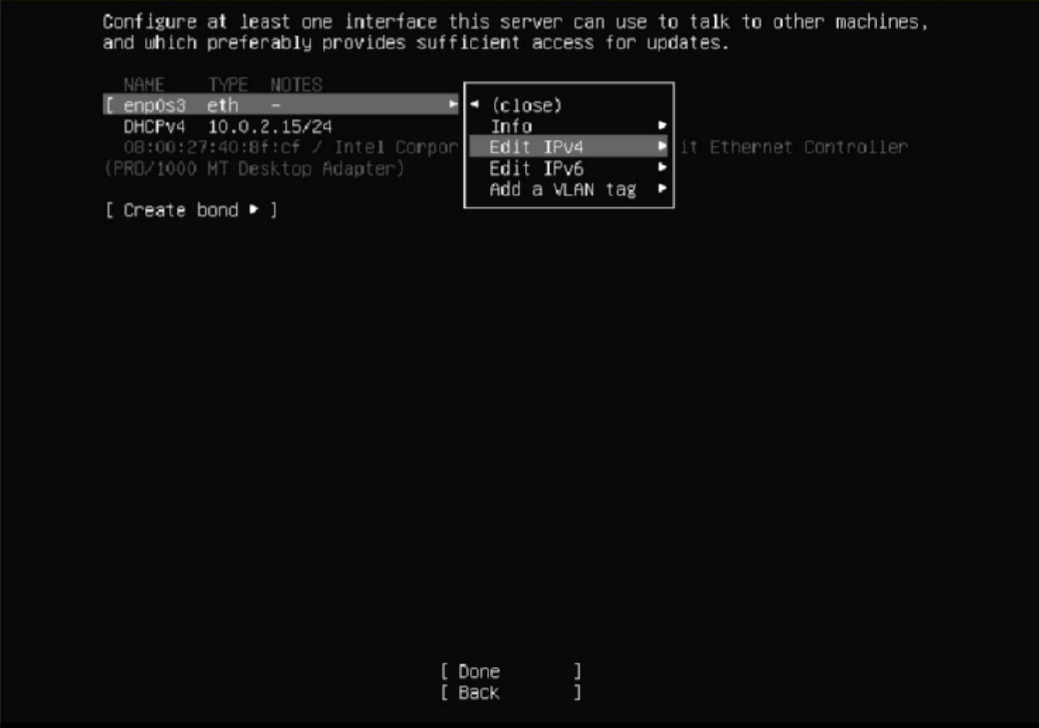
\includegraphics[width=1\textwidth]{imgs/1.3.png}}
    \label{1.3} %framework,fig1
\end{figure}

\begin{figure}[h]%current location
    \centering
    \scalebox{0.8}{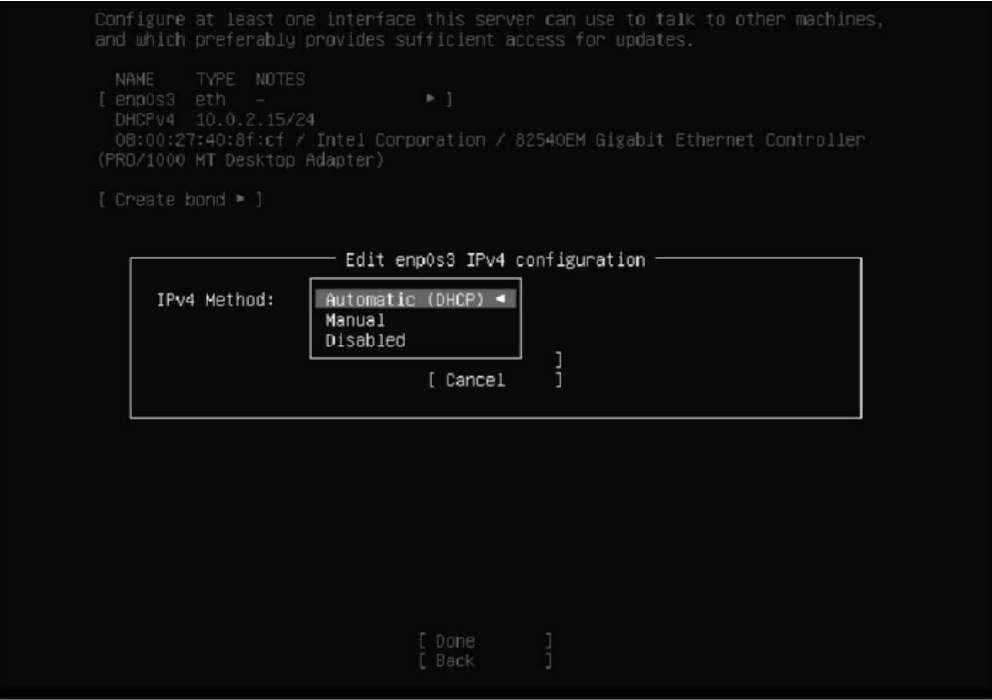
\includegraphics[width=1\textwidth]{imgs/1.4.png}}
    \label{1.4} %framework,fig1
\end{figure}

В большинстве случаев в домашнем окружении работает роутер, назначающий IP адреса с
помощью протокола DHCP, поэтому если в типе сетевого подключения (VirtualBox или VmWare Player)
установлен Bridge, виртуальная машина также получит IP адрес от домашнего роутера. Если в
качестве сетевого подключения используется NAT, адрес будет назначен из собственной подсети
среды виртуализации. Переходим к следующему шагу.


\subsection*{Разметка диска. Завершение установки ОС}
\addcontentsline{toc}{subsection}{Разметка диска. Завершение установки ОС}

Прежде чем провести разметку диска на разделы, разберём структуру файловой системы в
Linux. Файловая система Linux, в отличие от Windows, имеет древовидную структуру. Есть корневой
раздел (/ -root), в котором содержатся файлы и каталоги, которые в свою очередь могут быть точками
монтирования для других разделов.

Чтобы система загрузилась, зачастую достаточно двух разделов: корневого раздела «/» и
раздела SWAP.

SWAP — один из механизмов виртуальной памяти, при котором отдельные фрагменты памяти
(обычно неактивные) перемещаются из ОЗУ во вторичное хранилище (отдельный раздел или файл),
освобождая ОЗУ для загрузки других активных фрагментов памяти. Если мы разворачиваем сервер
под Kubernetes, то раздел SWAP не нужен.

Если нет каких-то особых требований, можно доверить разметку диска инсталлятору, но на
практике часто бывают случаи, когда разметка, предлагаемая инсталлятором, не удовлетворяет
требованиям к серверу, например, домашний каталог пользователей должен иметь иной тип
файловой системы. Второе отличие серверного варианта Ubuntu от десктопного — разметка дисков
осуществляется вручную.

В меню Filesystem setup выбираем диск и нажимаем Enter, появляется меню разметки:

\begin{figure}[H]%current location
    \centering
    \scalebox{0.9}{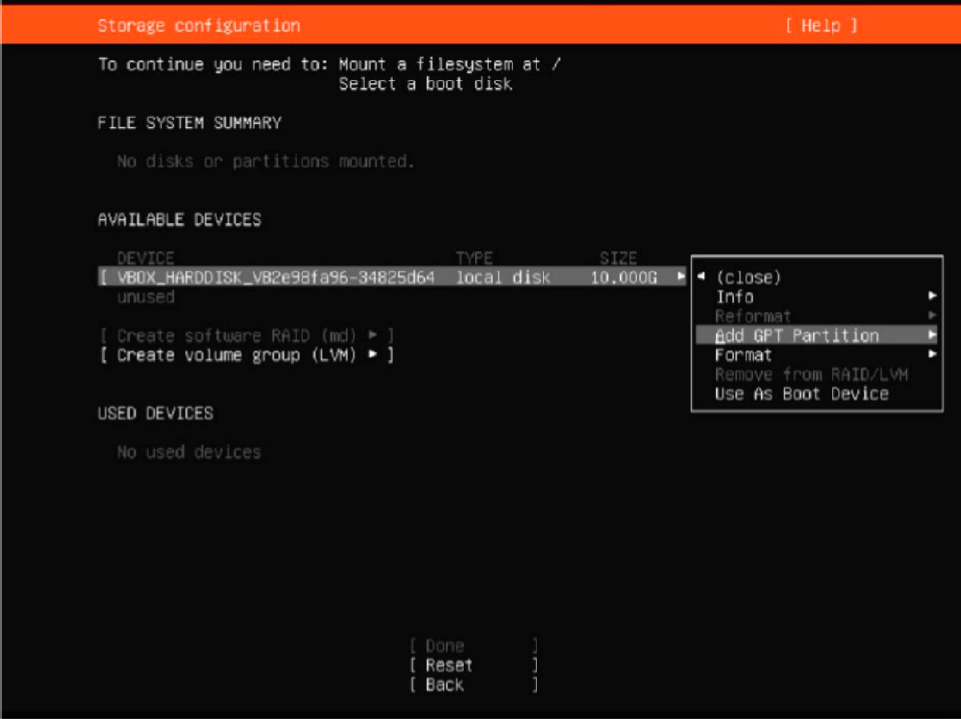
\includegraphics[width=1\textwidth]{imgs/1.5.png}}
    \label{1.5} %framework,fig1
\end{figure}

Выбираем пункт Add Partition, нажимаем Enter и заполняем поля следующим образом:

\begin{enumerate}
    \item Size (размер в GB) — 1G — объём пространства под раздел.
    \item Format — ext4 — тип \href{https://losst.ru/tipy-fajlovyh-sistem-dlya-linux}{файловой системы}, в которой будет отформатирован раздел.
    \item Mount — /boot — точка монтирования. Раздел /boot содержит загрузочные файлы,
    необходимые для старта системы (загрузчик, ядро и т. д.). Его рекомендуется выносить в
    отдельный раздел, в частности, если мы используем \href{https://ru.wikipedia.org/wiki/LVM}{LVM} при разметке дисков, так как ни
    BIOS, ни EFI не умеют работать с LVM-разделами.
\end{enumerate}

\begin{figure}[H]%current location
    \centering
    \scalebox{1}{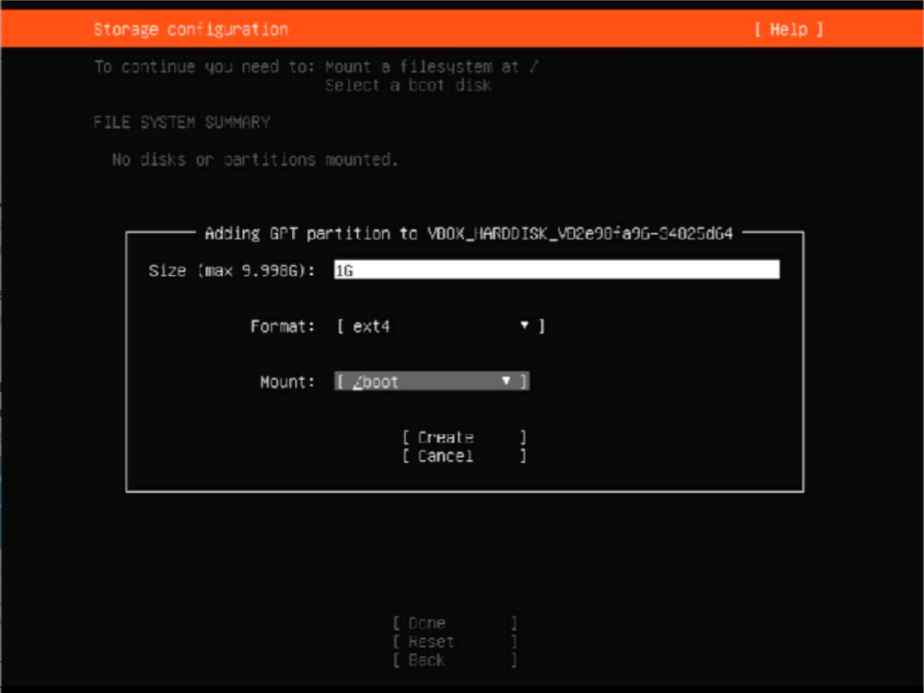
\includegraphics[width=1\textwidth]{imgs/1.6.png}}
    \label{1.6} %framework,fig1
\end{figure}

Прежде чем продолжить разбивку, дадим определение понятию LVM.

\href{https://help.ubuntu.ru/wiki/lvm}{Logical Volume Manager (LVM)} — это система управления томами с данными для Linux. Она
позволяет создавать поверх физических разделов или даже неразмеченных жёстких дисков
логические тома, которые в самой системе будут видны как обычные блочные устройства с данными,
то есть как обычные разделы. Рекомендуется использовать её в случае установки серверной версии
Ubuntu, так как она позволяет более гибко работать с имеющимся дисковым пространством:
увеличить или уменьшить раздел без потери данных и с минимальным простоем системы.

Оставшиеся разделы разметим с использованием LVM. Для этого выбираем свободное
пространство, нажимаем Enter. В пункте Size либо ничего не указываем (инсталлятор использует всё
доступное пространство), либо указываем размер. Тип файловой системы выбираем «Оставить
неформатированным» (Leave unformatted) и нажимаем Create.

\begin{figure}[H]%current location
    \centering
    \scalebox{0.75}{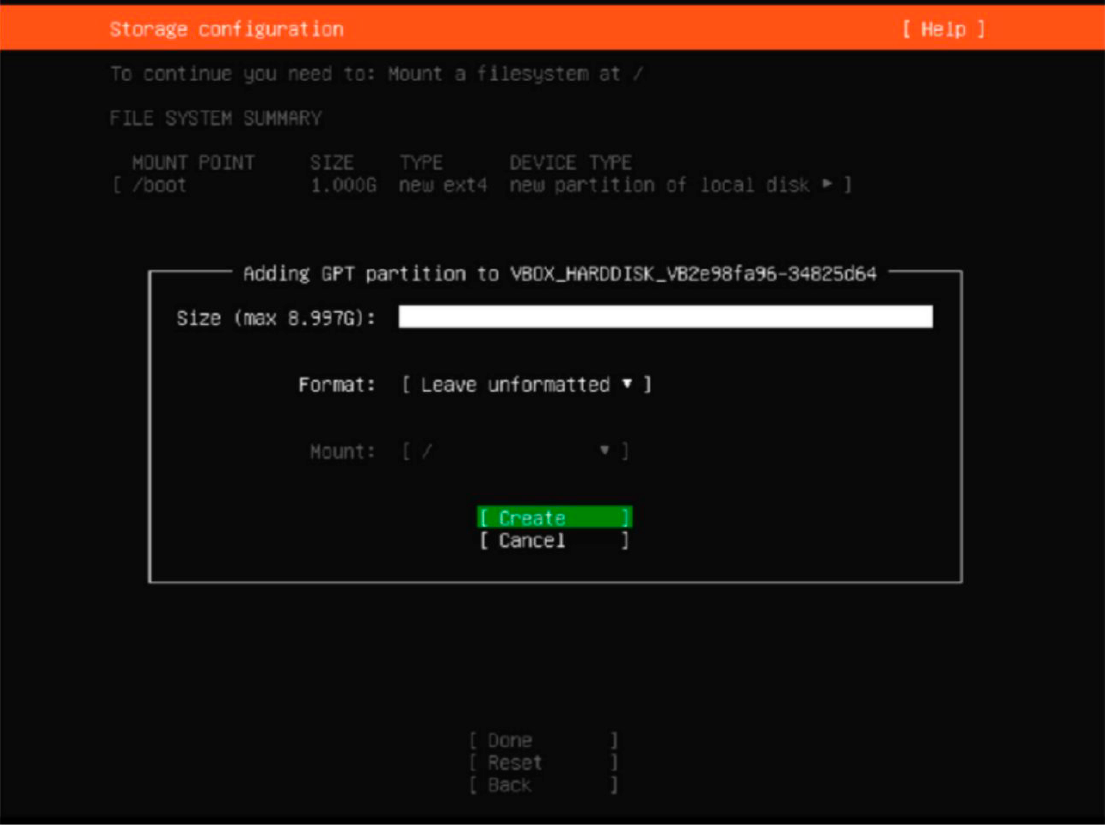
\includegraphics[width=1\textwidth]{imgs/1.7.png}}
    \label{1.7} %framework,fig1
\end{figure}

Следующий шаг: создаём Volume Group. Выбираем пункт Create volume group, нажимаем
Enter, имя группы оставляем по умолчанию и нажимаем Create. Volume Group с точки зрения LVM —
это абстракция, которая объединяет в себе физические тома (реальные жёсткие диски). В результате
мы получаем единое дисковое пространство, которое уже можем разбивать на своё усмотрение. В
меню разметки выбираем имя группы и нажимаем Enter. Открывается меню, в котором нас интересует
пункт Create Logical Volume.

\begin{figure}[h]%current location
    \centering
    \scalebox{0.75}{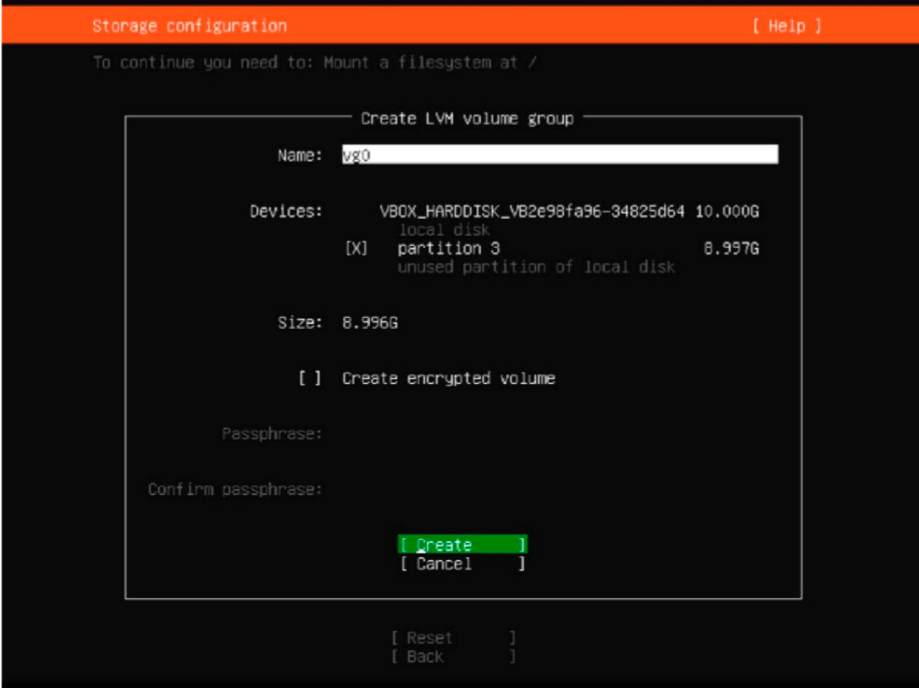
\includegraphics[width=1\textwidth]{imgs/1.8.png}}
    \label{1.8} %framework,fig1
\end{figure}

Создаём первый Logical Volume. С точки зрения операционной системы это обычный раздел.
Этот раздел в нашем случае будет \href{https://help.ubuntu.ru/wiki/swap}{SWAP}. Есть несколько подходов к выбору раздела SWAP:
\begin{enumerate}
    \item Самый распространённый: SWAP равен количеству оперативной памяти.
    \item Второй подход основан на \href{http://www.dba-oracle.com/t_linux_installation.htm}{рекомендации компании Oracle}: если в системе до 16 GiB
    оперативной памяти, то размер SWAP выставляем равным объёму ОЗУ, если выше 16 GiB, то
    размер SWAP равен 16 GiB.
    \item И третий подход: если мы готовим систему под кластер Kubernetes, то раздел SWAP вообще
    не нужен.
\end{enumerate}
В нашем случае выставляем размер раздела равным количеству оперативной памяти,
выделенной виртуальной машине:
\begin{figure}[h]%current location
    \centering
    \scalebox{0.9}{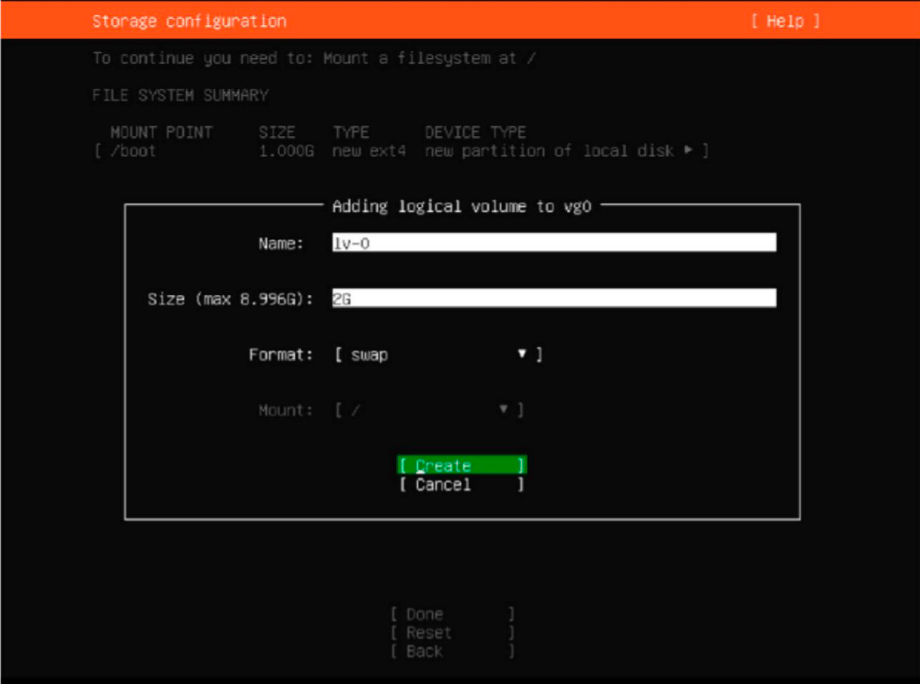
\includegraphics[width=1\textwidth]{imgs/1.9.png}}
    \label{1.9} %framework,fig1
\end{figure}
И завершаем разметку диска разделом «/», под который отдаём всё оставшееся место. Для
этого повторяем те же шаги, что и для раздела SWAP.
\begin{figure}[H]%current location
    \centering
    \scalebox{0.9}{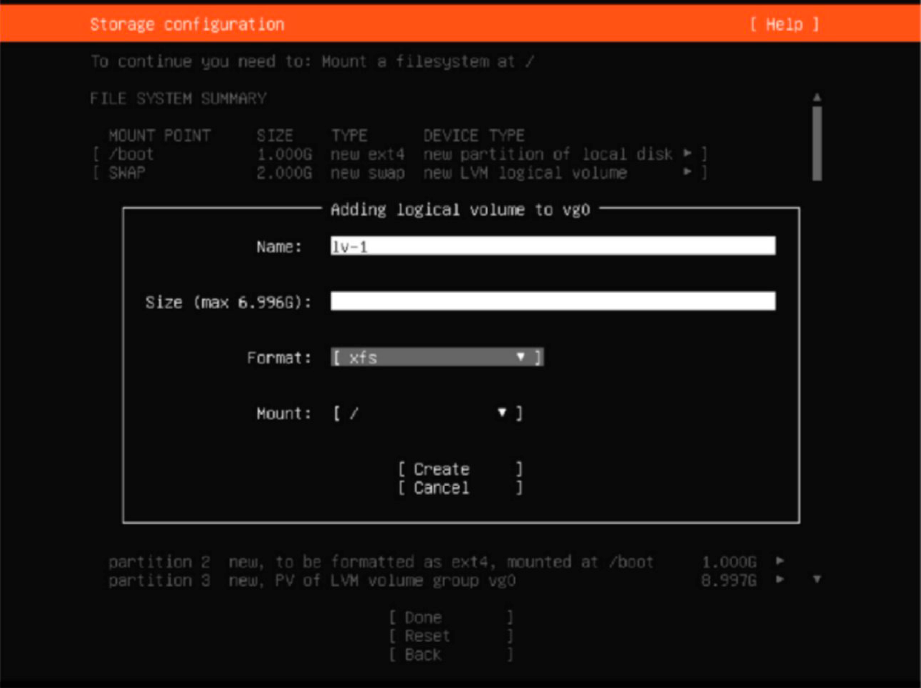
\includegraphics[width=1\textwidth]{imgs/1.10.png}}
    \label{1.10} %framework,fig1
\end{figure}
Заканчиваем разметку, нажав «Готово», и далее выбираем пункт «Продолжить»:
\begin{figure}[H]%current location
    \centering
    \scalebox{0.9}{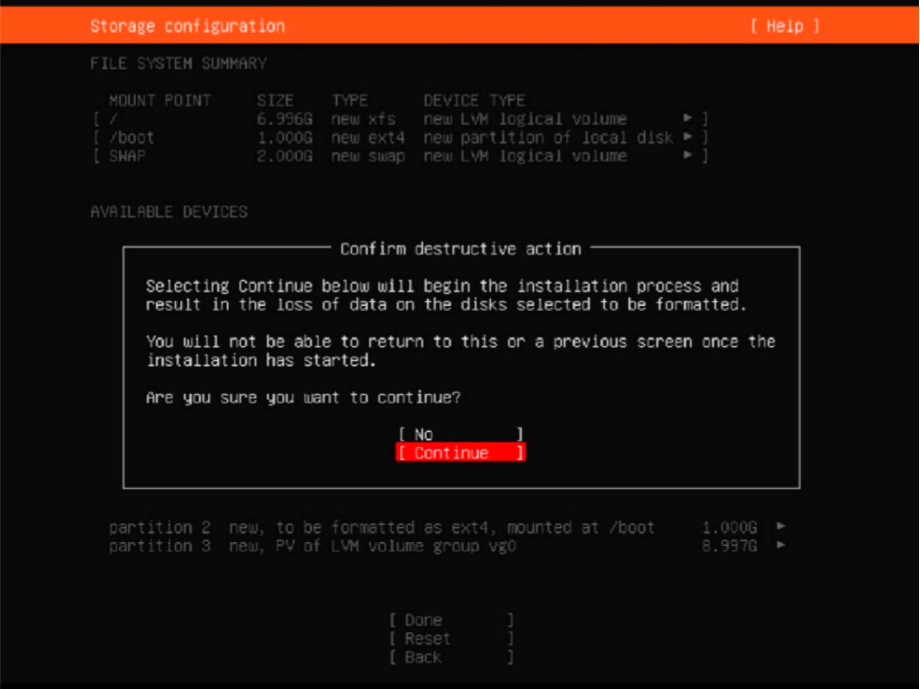
\includegraphics[width=1\textwidth]{imgs/1.11.png}}
    \label{1.11} %framework,fig1
\end{figure}


\subsection*{Создание пользователя}
\addcontentsline{toc}{subsection}{Создание пользователя}
После этого переходим к завершению установки. Создаём пользователя, который
будет основным пользователем системы или администратором компьютера, задаём пароль,
задаём имя сервера:
\begin{figure}[H]%current location
    \centering
    \scalebox{0.9}{
\includegraphics[width=1\textwidth]{imgs/1.12.png}}
    \label{1.12} %framework,fig1
\end{figure}
Следующий шаг — настройка SSH. В нашем случае мы активируем только пункт Install SSH
server:
\begin{figure}[H]%current location
    \centering
    \scalebox{0.9}{
\includegraphics[width=1\textwidth]{imgs/1.13.png}}
    \label{1.13} %framework,fig1
\end{figure}
Далее нам предлагается установить дополнительные возможности для сервера, этот пункт
пропускаем, жмём «Готово» и дожидаемся окончания установки ОС.
\begin{figure}[H]%current location
    \centering
    \scalebox{0.9}{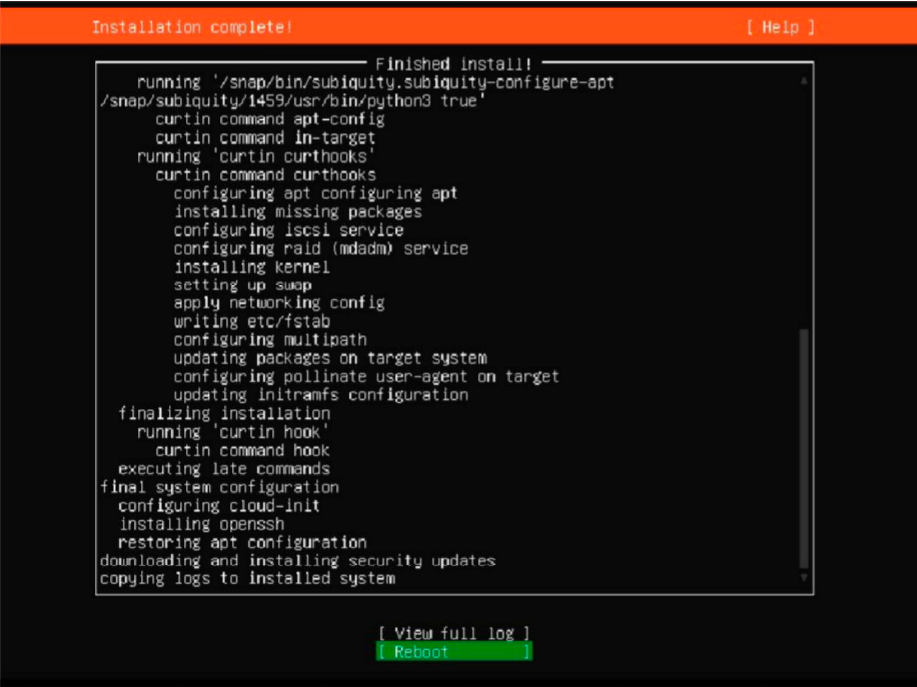
\includegraphics[width=1\textwidth]{imgs/1.14.png}}
    \label{1.14} %framework,fig1
\end{figure}


\subsection*{Обновление системы. Установка дополнений VM в случае необходимости}
\addcontentsline{toc}{subsection}{Обновление системы. Установка дополнений VM в случае необходимости}
Следующий шаг, который необходимо сделать после установки операционной системы, —
установить дополнения для виртуальной машины и обновить операционную систему. Дополнения, в
частности, необходимы, если мы используем виртуальную машину под управлением VirtualBox.

\subsubsection*{Установка дополнений гостевой ОС (VirtualBox)}
\addcontentsline{toc}{subsubsection}{Установка дополнений гостевой ОС (VirtualBox)}
Дополнения гостевой ОС содержат в себе набор приложений и драйверов, необходимых для
оптимизации, повышения производительности и удобства эксплуатации ОС.
%%%%%%%%%%%%%%%%%%%%%%%%%%%%%%%%%%%%%%%%%%%%%%%%%%%%%%%%%%%%%%%%%%%%%%%%%%%%%%%%%%%%%%%%%%%%%%%%%%%%%%%%%%%%%%%%%%%%%%%
\begin{enumerate}
    \item В меню управления виртуальной машиной выбираем пункт «Устройства» и в конце списка
    нажимаем «Подключить образ дополнений гостевой ОС».
    \item Установка приложений требует прав суперпользователя, поэтому все последующие действия
    будем совершать, используя утилиту sudo. В установленной ОС выполняем следующую
    команду: \colorbox{backcolour}{sudo apt update}. Apt — это утилита для управления пакетами, иными словами,
    приложениями в Ubuntu. Параметр \colorbox{backcolour}{update} говорит утилите, что необходимо обновить
    информацию о доступных пакетах в репозиториях (репозиторий — хранилище пакетов).
    \item Используя утилиту apt, скачаем и установим следующие пакеты: sudo apt install perl
    make gcc -y. Здесь параметр install говорит утилите apt, что необходимо поставить три
    пакета, и параметр -y означает, что apt будет устанавливать пакеты без подтверждения от
    пользователя.
    \item В Ubuntu Server не включена функция автомонтирования (подключения) внешних носителей.
    Следующий шаг — монтируем подключенный образ дополнений в ОС (требует прав
    суперпользователя): \colorbox{backcolour}{sudo mount /dev/cdrom /mnt} , где \colorbox{backcolour}{mount} — утилита монтирования
    дисковых устройств в Linux, \colorbox{backcolour}{/dev/cdrom} — это виртуальное устройство чтения
    компакт-дисков. Оно же может быть и реальным, физическим. Каталог \colorbox{backcolour}{/mnt} — точка
    монтирования \colorbox{backcolour}{cdrom}.
    \item Переходим в каталог /mnt: \colorbox{backcolour}{cd /mnt}. cd (Change Directory) — команда для перемещения между
    каталогами в Linux. Запускаем скрипт установки дополнений: \colorbox{backcolour}{sudo
    ./VBoxLinuxAdditions.run}.
\end{enumerate}

После установки дополнений необходимо перезагрузить операционную систему, но, прежде
чем это сделать, необходимо установить обновления. Для этого выполним команду \colorbox{backcolour}{sudo apt
upgrade -y} . Параметры \colorbox{backcolour}{upgrade -y} передают утилите apt, что нужно провести обновление
системы, не спрашивая подтверждения у пользователя. По завершении обновления перезагружаем
ОС: \colorbox{backcolour}{sudo reboot}.



\subsection*{Установка OpenSSH Server и файлового менеджера
Midnight Commander}
\addcontentsline{toc}{subsection}{Установка OpenSSH Server и файлового менеджера
Midnight Commander}
В Ubuntu Server OpenSSH Server ставится автоматически, в случае использования Ubuntu
Desktop его необходимо установить самостоятельно: \colorbox{backcolour}{sudo apt install openssh-server -y}.
Также для удобства навигации и работы с файлами рекомендуется поставить файловый менеджер
Midnight Commander: \colorbox{backcolour}{sudo apt install mc -y}.\newpage


\section*{Практическое задание}
\addcontentsline{toc}{section}{Практическое задание}
При работе над практическим заданием:
\begin{enumerate}
    \item Установить VMWare Player/Virtualbox, установить Ubuntu.
    \item[2*.] Установить утилиты для гостевой ОС.
\end{enumerate}\newpage

\section*{Глоссарий}
\addcontentsline{toc}{section}{Глоссарий}
\href{https://ru.wikipedia.org/wiki/Âèðòóàëèçàöèÿ}{Виртуализация} — предоставление набора вычислительных ресурсов или их логического
объединения, абстрагированное от аппаратной реализации, и обеспечивающее при этом логическую
изоляцию друг от друга вычислительных процессов, выполняемых на одном физическом ресурсе.

\href{https://ru.wikipedia.org/wiki/Âèðòóàëüíàÿ_ìàøèíà}{Виртуальная машина} — программная и/или аппаратная система, эмулирующая аппаратное
обеспечение некоторой платформы (target — целевая, или гостевая платформа) и исполняющая
программы для target-платформы на host-платформе (host — платформа-хозяин) или
виртуализирующая некоторую платформу и создающая на ней среды, изолирующие друг от друга
программы и даже операционные системы.

\href{https://www.virtualbox.org/}{VirtualBox} (Oracle VM VirtualBox) — программный продукт виртуализации для операционных систем
Microsoft Windows, Linux, FreeBSD, macOS.

\href{https://www.vmware.com/ru/products/workstation-player.html}{VMWare Player} (VMware Workstation Player) — бесплатный для некоммерческого использования
программный продукт на основе виртуальной машины VMware Workstation, но с ограниченной
функциональностью, предназначенный для запуска образов виртуальных машин.

\href{https://help.ubuntu.ru/wiki/ðàçäåëû_è_ôàéëîâûå_ñèñòåìû_linux}{Раздел} — часть долговременной памяти жёсткого диска или флеш-накопителя, выделенная для
удобства работы и состоящая из смежных блоков. На одном устройстве хранения может быть
несколько разделов.

\href{https://help.ubuntu.ru/wiki/lvm}{Logical Volume Manager (LVM)} — система управления томами с данными для Linux. Она позволяет
создавать поверх физических разделов (или даже неразбитых жёстких дисков) логические тома,
которые в самой системе будут видны как обычные блочные устройства с данными, то есть как
обычные разделы.

\href{https://ru.wikipedia.org/wiki/Bash}{Bash} (сокр. от англ. Bourne again shell, каламбур «Born again» shell — «возрождённый» shell) —
усовершенствованная и модернизированная вариация командной оболочки Bourne shell. Одна из
наиболее популярных современных разновидностей командной оболочки UNIX. Особенно популярна
в среде Linux, где она часто используется в качестве предустановленной командной оболочки.

\href{https://ru.wikipedia.org/wiki/IP-%D0%B0%D0%B4%D1%80%D0%B5%D1%81}{IP-адрес} — уникальный сетевой адрес узла в компьютерной сети, построенной на основе стека
протоколов TCP/IP.

\section*{Дополнительные материалы}
\addcontentsline{toc}{section}{Дополнительные материалы}
\begin{enumerate}
    \item \href{https://losst.ru/ustanovka-centos-7}{https://losst.ru/ustanovka-centos-7}
    \item Уорд Б. Внутреннее устройство Linux. — СПб.: Питер, 2016. — 384 с.: ил. — (Серия «Для
    профессионалов»). ISBN 978-5-496-01952-1
    \item Немет, Эви, Снайдер, Гарт, Хейн, Трент, Уэйли, Бэн. Unix и Linux: руководство системного
    администратора, 4-е изд. : Пер. с англ. — М.: ООО «И.Д. Вильямс», 2012. — 1312 с.: ил. —
    Парал. тит. англ. ISBN 978-5-8459-1740-9 (рус.)
    \item Дэвид Даймонд, Линус Торвальдс. Just for fun. Рассказ нечаянного революционера.
    \href{https://v.gd/just_for_fun}{https://v.gd/just\_for\_fun}
    \item \href{https://upload.wikimedia.org/wikipedia/commons/7/77/Unix_history-simple.svg}{Дерево развития UNIX-подобных систем}.
\end{enumerate}

\section*{Используемые источники}
\addcontentsline{toc}{section}{Используемые источники}
\begin{enumerate}
    \item https://help.ubuntu.com/20.04/installation-guide/amd64/install.en.pdf
    \item \href{https://losst.ru/kak-polzovatsya-virtualbox}{https://losst.ru/kak-polzovatsya-virtualbox} — как пользоваться VirtualBox.
\end{enumerate}

\end{document}